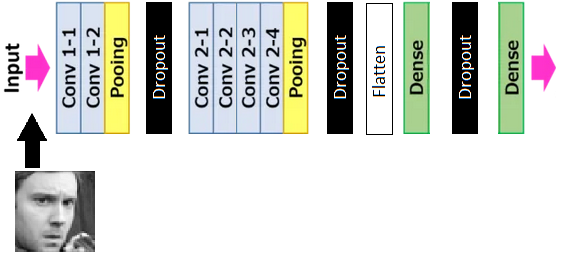
\includegraphics[scale=1]{images/modelTwo/modelImg.png}
Similar to the vgg16 model, new model will only use very small (3x3) filters in convolutional layers. The input will consist of array with a size of 48 by 48. Two layers followed by max Pooling layer with filter size 2x2 and by Dropout layer. Next step is four more convolutional layers, followed by the same two layers are previous step. Then, flatten output and pass it to two more layers.

It gives slightly more than 22 million of trainable parameters, previous model had ~15 millions of parameters, most of them pre-trained.